\documentclass[a4paper, 11pt]{article}
%\documentclass[a4paper, 12pt]{article}[abntex2]
%\documentclass[a4paper, 12pt, article]{abntex2}
%\setlrmarginsandblock{3cm}{2cm}{*}
%\setulmarginsandblock{3cm}{2cm}{*}
%\checkandfixthelayout
%\usepackage[alf]{abntex2cite}
\usepackage[brazil]{babel}
\usepackage[utf8]{inputenc}
\usepackage{amsmath}
\usepackage{indentfirst}
\usepackage{graphicx,color}
\usepackage{multicol,lipsum}
\usepackage[top=3cm,bottom=2cm,left=3 cm,right=2cm]{geometry}
\usepackage{esvect}
\usepackage{setspace}
\usepackage{subcaption}
\usepackage{textcomp}
\usepackage{fontenc}[T1]
\usepackage{gensymb}
\usepackage{wasysym}
\setstretch{1.5}
\usepackage[table,xcdraw]{xcolor}
\usepackage{colortbl}
\usepackage{caption}
\usepackage{float}
\usepackage[pdftex]{hyperref}
\bibliographystyle{acm}

\usepackage{listings}
\usepackage{xcolor}


\geometry{
    top=3cm,     % Margem superior
    bottom=2cm,  % Margem inferior
    left=2.5cm,  % Margem esquerda
    right=2.5cm  % Margem direita
}

\lstset{
    language=Python,
    basicstyle=\ttfamily\small,
    keywordstyle=\color{blue}\bfseries,
    stringstyle=\color{red},
    commentstyle=\color{gray},
    numbers=left,
    numberstyle=\tiny\color{gray},
    frame=single,
    breaklines=true,
    tabsize=1,
    showspaces=false,
    showstringspaces=false
}

\bibliographystyle{acm}

\begin{document}

\begin{titlepage}
	\begin{center}
	\begin{figure}[!ht]
	\centering
	
\includegraphics[width=6cm]{imgs/LNCC.png}
	\end{figure}
		LABORATÓRIO NACIONAL DE COMPUTAÇÃO CIENTÍFICA\\
		MESTRADO EM MODELAGEM COMPUTACIONAL\\ 
		\vspace{7cm}
		{\Large \textbf{Trabalho (GA030 - Estatística)}}
		\vspace{3cm}
	\end{center}
	
	\begin{flushright}
            Lorran de Araújo Durães Soares\\
	 \end{flushright}

	\begin{center}
		\vspace{\fill}
		 Petrópolis - RJ\\
         2024
	\end{center}
\end{titlepage}

\begin{titlepage}
	\begin{center}
        Lorran de Araújo Durães Soares \\
      \vspace{7cm}
      {\Large \textbf{Trabalho (GA030 - Estatística)}}
	\end{center}
\vspace{3cm}
	\begin{flushright}
   \begin{list}{}{
      \setlength{\leftmargin}{5cm}
      \setlength{\rightmargin}{0cm}
      \setlength{\labelwidth}{0pt}
      \setlength{\labelsep}{\leftmargin}}
      \begin{flushright}
          \item Trabalho  apresentado  como  parte  dos  critérios 
de avaliação da disciplina GA030 - Estatística.
       \item Professor(a): Marcio Rentes Borges
      \end{flushright}
      
   \end{list}
	\end{flushright}

	\begin{center}
		\vspace{\fill}
		 Petrópolis - RJ\\
         2024
	\end{center}
\end{titlepage}

\tableofcontents
\newpage

\section{\textbf{Introdução}}

Este texto refere-se ao trabalho realizado na disciplina GA030 (Estatística), do curso de pós-graduação oferecido pelo Laboratório Nacional de Computação Científica (LNCC), sob a orientação do professor Marcio Rentes Borges. Neste documento, serão apresentadas as questões propostas pelo trabalho, seguidas de suas respectivas resoluções. \href{https://github.com/lorran-araujo/LNCC/blob/main/disciplinas/estatistica/trab1/trab.ipynb}{Clique aqui} para acessar o código referente à realização de todos os exercícios.

\section{\textbf{Questão 1}}
\noindent Após abordarmos a \textit{Lei dos Grandes Números} e o \textit{Teorema do Limite Central}, chegamos a um ponto crucial do curso: a estimação de parâmetros (desconhecidos) associados à distribuição de probabilidade de uma variável aleatória.

\noindent O presente trabalho tem como objetivo a fixação das ideias introduzidas até aqui. Para isso, utilizaremos dados armazenados em quatro arquivos, que contêm amostras de diferentes variáveis aleatórias, conforme a Tabela 1.

\begin{table}[H]
    \centering
    \begin{tabular}{|c|c|c|}
        \hline
        \textbf{Variável} & \textbf{Arquivo} & \textbf{Distribuição} \\
        \hline
        $Q \sim \mathcal{N}(0, 2)$ & \texttt{data1q.dat} & Normal \\
        $X \sim U[-1, 1]$ & \texttt{data1x.dat} & Uniforme \\
        $Y \sim E(\lambda = 0.05)$ & \texttt{data1y.dat} & Exponencial \\
        $T \sim B(15, 0.40)$ & \texttt{data1t.dat} & Binomial \\
        \hline
    \end{tabular}
    \caption{Tabela de dados}
    \label{tab:dados}
\end{table}

\subsection{\textbf{(a)}}

\noindent Dado que conhecemos a distribuição de probabilidades de cada variável aleatória e os parâmetros que as caracterizam (Tabela \ref{tab:dados}), calcule a expectativa e a variância (teóricas) de cada uma delas, usando as definições que vimos em aula.

\textbf{Resolução:}

Usando as definições dadas em aula \cite{borges_site} e utilizando os parâmetros presentes na tabela \ref{tab:dados}, iremos calcular a média e a variância teórica de cada variável aleatória:

\begin{itemize}
    \item Para a variável $Q$, não será necessário cálculos, pois os próprios parâmetros da curva normal fornecem à sua média e variância. Logo, $\mu_Q = 0$ e ${{\sigma}_Q}^{2} = 2$.
    
    \item Para a variável $X$, que tem origem em uma distribuição uniforme, teremos que a média e a variância serão dadas por:
    \[
    \mu_X = \dfrac{-1+1}{2} \Rightarrow \mu_X = 0
    \]
    \[
    {{\sigma}_X}^{2} = \dfrac{{(1-(-1))}^2}{12}=\dfrac{4}{12} \Rightarrow {{\sigma}_X}^{2} = \dfrac{1}{3}
    \]

    \item Para a variável $Y$, originado através de uma distribuição exponencial com $\lambda=0.05$, teremos que a média e a variância serão dadas por:
    \[
    \mu_Y = \dfrac{1}{\lambda} = \dfrac{1}{0.05} \Rightarrow \mu_y = 20
    \]
    \[
    {{\sigma}_Y}^{2} = \dfrac{1}{\lambda^2} = \dfrac{1}{0.05^2} = \dfrac{1}{0.0025} \Rightarrow {{\sigma}_Y}^{2} = 400
    \]

    \item Para a variável $T$, dada por uma distribuição binomial com $p=0.40$ e $N=15$, teremos que a média e a variância serão dadas então por:
    \[
    \mu_T = N \cdot p = 15 \cdot 0.4 \Rightarrow \mu_T = 6
    \]
    \[
    {{\sigma}_T}^{2} = N\cdot p(1-p)=15 \cdot 0.4(1-0.4) \Rightarrow {{\sigma}_T}^{2} = 3.6
    \]
\end{itemize}

Logo, com os resultados obtidos, a tabela \ref{tab:medvar} apresenta a média e variância teóricas de cada uma das variáveis aleatórias.

\begin{table}[H]
    \centering
    \begin{tabular}{|c|c|c|}
        \hline
        \textbf{Variável} & \textbf{Média} & \textbf{Variância} \\
        \hline
        $Q \sim N(0, 2)$ & $0$ & $2$ \\
        $X \sim U[-1, 1]$ & $0$ & $\dfrac{1}{3}$ \\
        $Y \sim E(\lambda = 0.05)$ & $20$ & $400$ \\
        $T \sim B(15, 0.40)$ & $6$ & $3.6$ \\
        \hline
    \end{tabular}
    \caption{Média e Variância dos dados}
    \label{tab:medvar}
\end{table}

\subsection{\textbf{(b)}}

\noindent Utilize o R (ou outro programa) para ler cada arquivo e calcule estimativas para a
média e a variância do conjunto de dados (usando todos os dados disponíveis nos
arquivos). Em seguida, compare com os resultados obtidos no exercício anterior.
Faça comentários.

\textbf{Resolução:}

Para estimar a média e a variância de cada variável, utilizaremos os estimadores clássicos, pois eles são estimativas não tendenciosas, de variância mínima e consistentes:

\[
\bar{X} = \dfrac{1}{n} \sum_{i=1}^{n} X_i
\]

\[
S^2 = \dfrac{1}{n-1} \sum_{i=1}^{n} (X_i - \bar{X})^2
\]

Foi desenvolvido um programa em Python para calcular as estimativas da média e da variância de cada variável aleatória. Os resultados obtidos estão apresentados na Tabela \ref{tab:esti}, com precisão de três casas decimais.

\begin{table}[H]
    \centering
    \begin{tabular}{|c|c|c|}
        \hline
        \textbf{Variável} & \textbf{Média} & \textbf{Variância} \\
        \hline
        $Q \sim N(0, 2)$ & $ 0 $ & $2$ \\
        $X \sim U[-1, 1]$ & $0$ & $0.333$ \\
        $Y \sim E(\lambda = 0.05)$ & $20.007$ & $400.37$ \\
        $T \sim B(15, 0.40)$ & $6$ & $3.602$ \\
        \hline
    \end{tabular}
    \caption{Estimativas para a Média e Variância dos dados}
    \label{tab:esti}
\end{table}

A realização deste exercício revelou que as estimativas da média e da variância encontradas foram altamente precisas, aproximando-se dos valores reais teóricos. Essa precisão é garantida pelo grande número de amostras em cada conjunto de dados. Com 5 milhões de amostras por variável aleatória, é possível calcular a média e a variância com elevado grau de exatidão.

\subsection{\textbf{(c)}}

\noindent Construa os histogramas com as frequências relativas de cada uma das variáveis,
verificando se estes são condizentes com os modelos teóricos (Tabela 1).

\textbf{Resolução:}

Para cada variável aleatória, foi construído o histograma das frequências relativas, normalizado de forma que, devido à grande quantidade de dados, o histograma se aproximasse da função de densidade de probabilidade (PDF) ou da função de probabilidade (PMF) correspondente à distribuição teórica dos dados. Para verificar a consistência com o modelo teórico, a PDF ou PMF teórica foi sobreposta ao histograma. A Figura \ref{fig:hist} apresenta os resultados obtidos. No caso de variáveis contínuas, as partições (bins) foram ajustadas automaticamente.

\begin{figure}[H]
    \centering 
    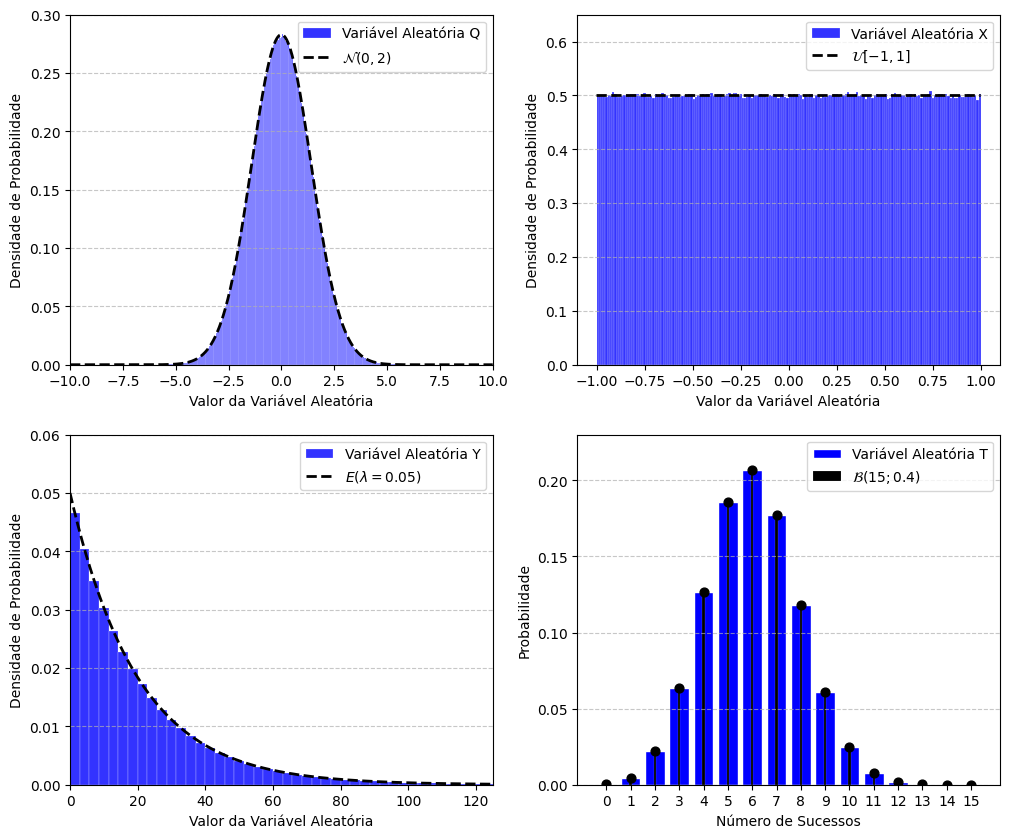
\includegraphics[width=0.9\textwidth]{imgs/hist.png}
    \caption{Histograma de frequências relativas dos dados com distribuições sobrepostas}
    \label{fig:hist} % cria um rótulo para referência no texto
\end{figure}

A análise da Figura \ref{fig:hist} demonstra que os histogramas estão alinhados com seus respectivos modelos teóricos, uma vez que os dados apresentaram um ajuste adequado às PDFs ou PMFs em todos os casos.

\subsection{\textbf{(d)}}

\noindent Considere cada uma das amostras das variáveis aleatórias, contidas nos arquivos, e suas diferentes distribuições de probabilidades. Tome amostras aleatórias de tamanho n (n = 5, 10 e 50) de cada uma das variáveis aleatórias e construa as variáveis aleatórias (estatísticas):

\begin{itemize}
    \item \textit{média amostral:} \[{\bar{W}}^{(n)}=\dfrac{1}{n} \sum_{i=1}^{n} W_i\]
    \item \textit{variância amostral:} \[{S_W}^{2(n)}=\dfrac{1}{n-1} \sum_{i=1}^{n}(W_i - \bar{W}_n)^2\]
\end{itemize}

onde $W = Q, X, Y$ ou $T$. Use 10000 amostras simples (pontos amostrais) para gerar
as variáveis aleatórias média amostral e variância amostral. Obs.: Lembre-se das
características que as amostras aleatórias devem ter. Apresente o código.

\textbf{Resolução:}

Para resolver esta questão, foram realizados 1000 sorteios aleatórios contendo 5, 10 e, posteriormente, 50 valores de cada variável aleatória. Com esses sorteios, foram construídas as variáveis aleatórias referentes à média amostral e à variância amostral utilizando as fórmulas descritas no enunciado da questão. A Figura \ref{fig:cod} apresenta o código utilizado para implementar esse procedimento.

\begin{figure}[H]
    \centering
    \begin{minipage}{\textwidth}
    \begin{lstlisting}
n_samples = [5,10,50]
        
for key, dat in data.items():
    for n in n_samples:
        medias = []
        variancias = []
        
        amostras = np.random.choice(dat, size=(10000, n), replace=False)
        medias = amostras.mean(axis=1)
        variancias = amostras.var(axis=1, ddof=1)
        
        if key == 'data_q':
            medias_amostrais_q[f'{key}_{n}'] = medias
            variancias_amostrais_q[f'{key}_{n}'] = variancias
        elif key == 'data_x':
            medias_amostrais_x[f'{key}_{n}'] = medias
            variancias_amostrais_x[f'{key}_{n}'] = variancias
        elif key == 'data_y':
            medias_amostrais_y[f'{key}_{n}'] = medias
            variancias_amostrais_y[f'{key}_{n}'] = variancias
        elif key == 'data_t':
            medias_amostrais_t[f'{key}_{n}'] = medias
            variancias_amostrais_t[f'{key}_{n}'] = variancias
        else:
            raise(ValueError)
    \end{lstlisting}   
    \end{minipage} 
    \caption{Código para cálculo das variáveis média amostral e variância amostral}
    \label{fig:cod}
\end{figure}


\subsection{\textbf{(e)}}

\noindent Usando o código da questão anterior, construa os histogramas de frequências das
variáveis aleatórias média amostral e variância amostral, para os diferentes valores de n e compare com as distribuições teóricas esperadas para estas variáveis.
Faça isso para as variáveis (Q, X, Y e T).

\textbf{Resolução:}

Para esta questão, espera-se que as médias amostrais sigam uma distribuição normal, com a mesma média da variável de origem e com variância igual à variância da variável aleatória de origem dividida por \( n \), onde \( n \) representa o número de amostras que compõem a média amostral (neste caso, \( n = 5 \), \( n = 10 \) ou \( n = 50 \)). 

No caso da variância, para variáveis originadas de distribuições normais, ao ser multiplicada pelo fator $\dfrac{n-1}{\sigma^2}$, onde $\sigma^2$ é a variância da variável de origem, espera-se que ela siga uma distribuição qui-quadrado com \( n - 1 \) graus de liberdade. Para as demais variáveis, não há uma expectativa específica sobre o comportamento da variância amostral.

Dessa forma, foram construídos histogramas e sobrepostas as curvas teóricas esperadas. Os resultados estão apresentados nas Figuras \ref{fig:medvarQ}, \ref{fig:medvarX}, \ref{fig:medvarY} e \ref{fig:medvarT}. Cada coluna dessas figuras exibe o histograma da média amostral (em azul) e o da variância amostral (em vermelho) para \( n = 5 \), \( n = 10 \) e \( n = 50 \), respectivamente.

\begin{figure}[H]
    \centering 
    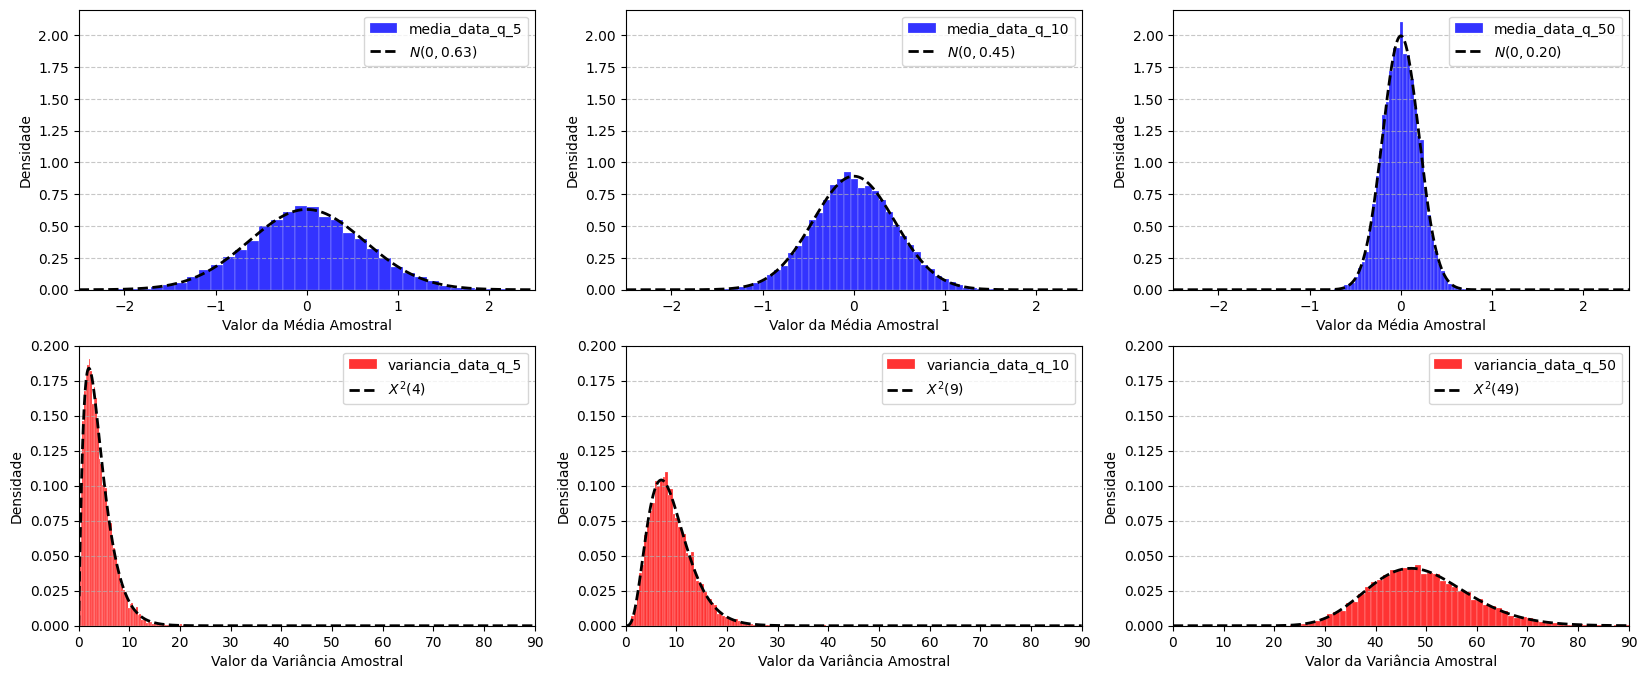
\includegraphics[width=1\textwidth]{imgs/medvarQ.png}
    \caption{Histograma das variáveis média e variância amostrais com origem Q}
    \label{fig:medvarQ} % cria um rótulo para referência no texto
\end{figure}

\begin{figure}[H]
    \centering 
    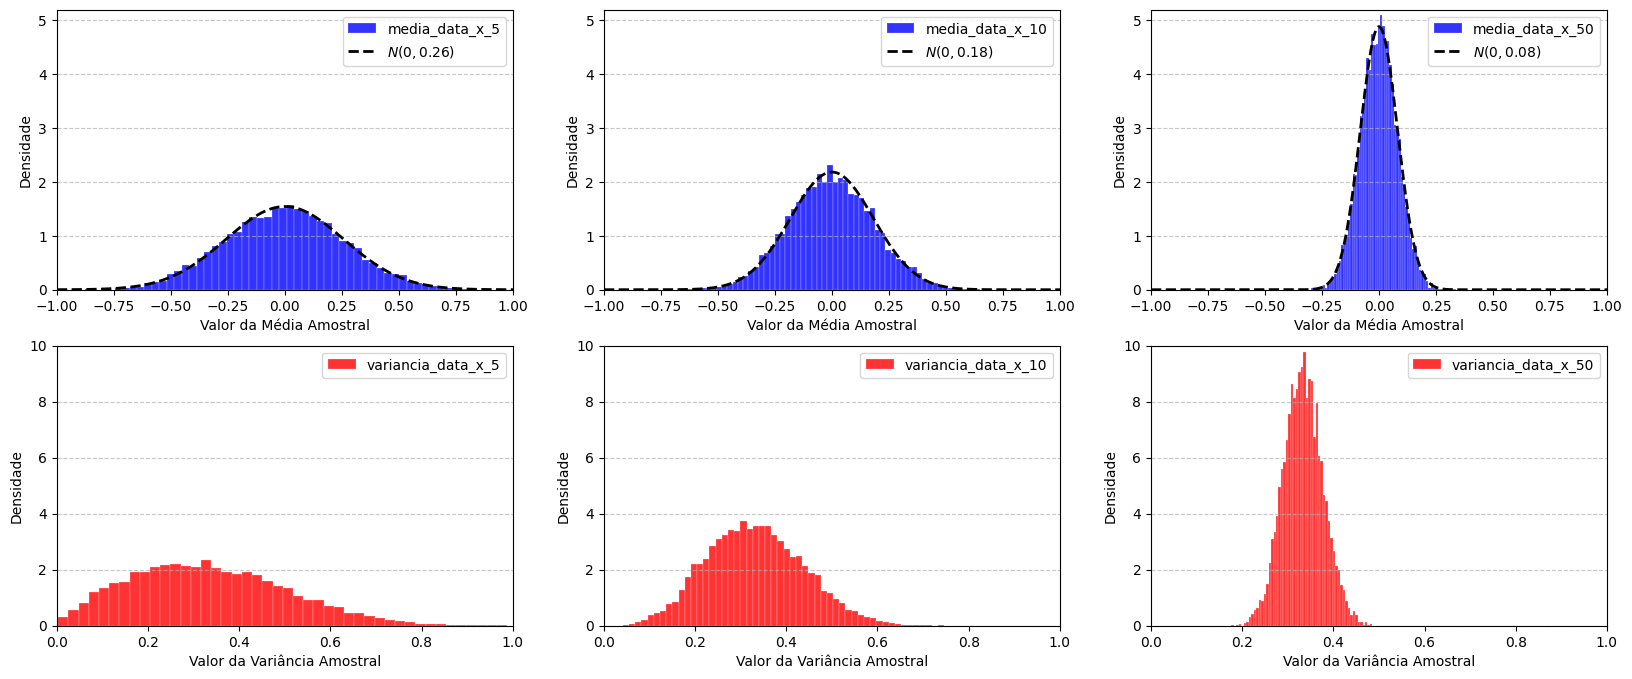
\includegraphics[width=1\textwidth]{imgs/medvarX.png}
    \caption{Histograma das variáveis média e variância amostrais com origem X}
    \label{fig:medvarX} % cria um rótulo para referência no texto
\end{figure}

\begin{figure}[H]
    \centering 
    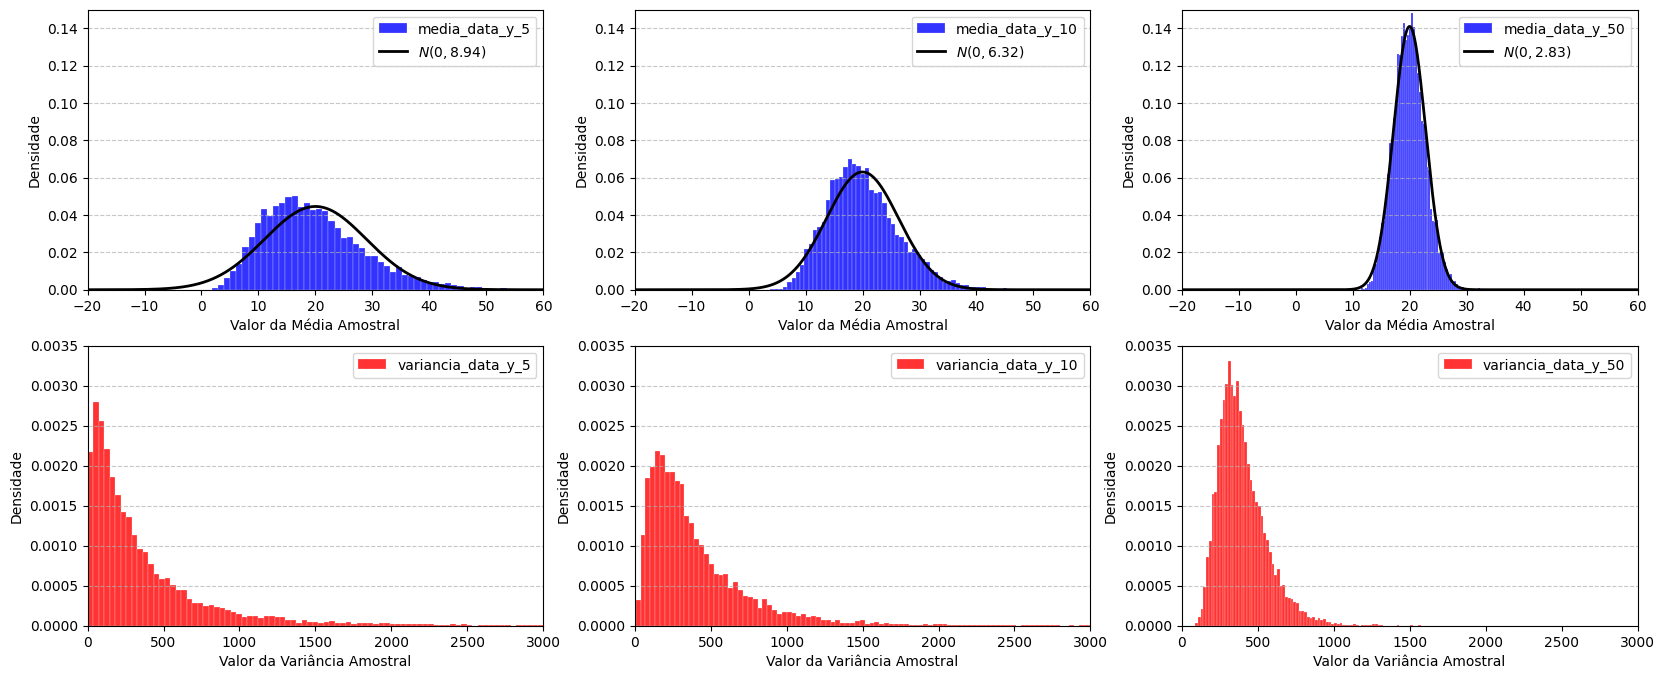
\includegraphics[width=1\textwidth]{imgs/medvarY.png}
    \caption{Histograma das variáveis média e variância amostrais  com origem Y}
    \label{fig:medvarY} % cria um rótulo para referência no texto
\end{figure}

\begin{figure}[H]
    \centering 
    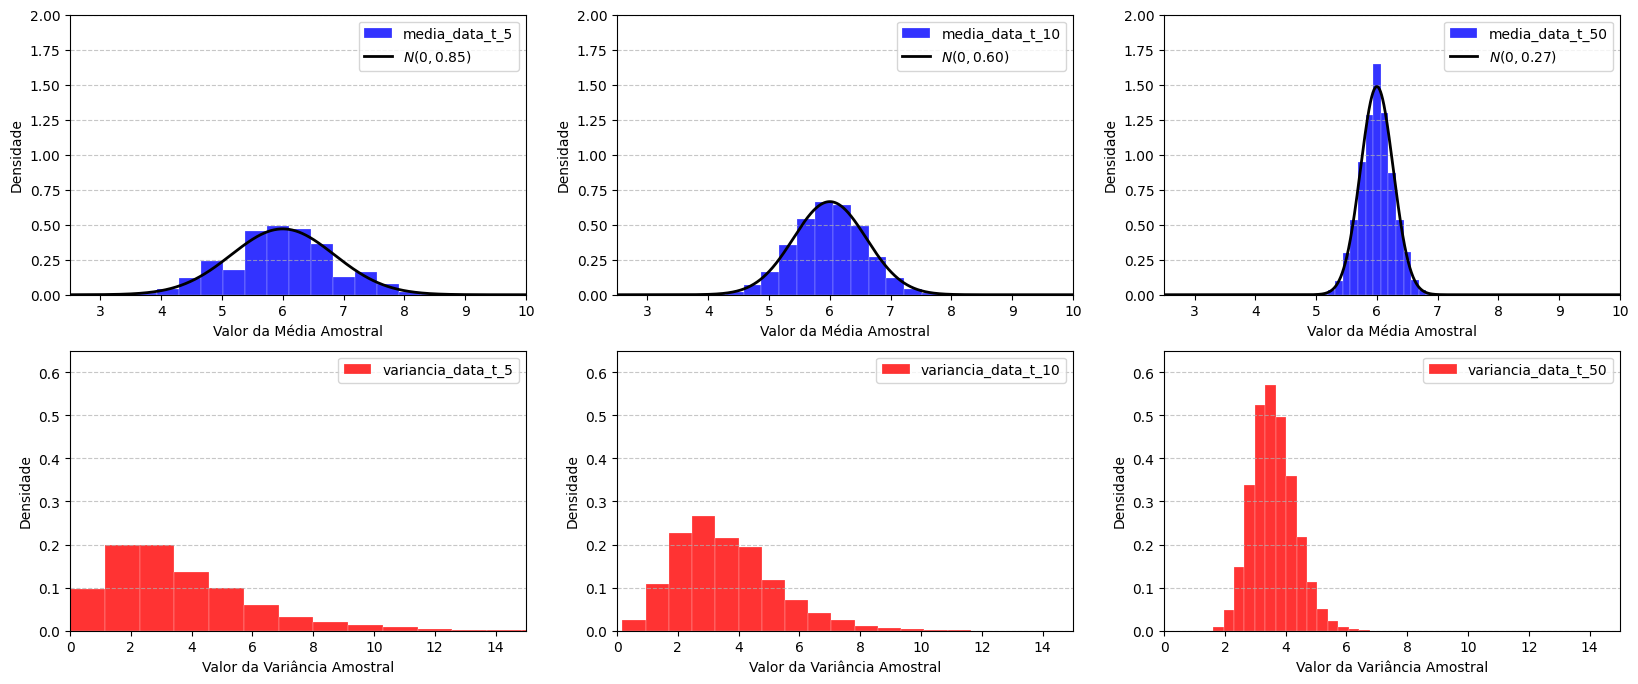
\includegraphics[width=1\textwidth]{imgs/medvarT.png}
    \caption{Histograma das variáveis média e variância amostrais com origem T}
    \label{fig:medvarT} % cria um rótulo para referência no texto
\end{figure}

Ao observar a sobreposição das curvas, nota-se que os histogramas se ajustam de forma satisfatória às distribuições teóricas esperadas para cada variável. 
Esse comportamento indica que as médias amostrais seguem uma distribuição aproximadamente normal, com a mesma média da variável original e variância reduzida por um fator de \( n \).

Além disso, a variância amostral, no caso da variável originada de uma distribuição normal, apresenta o comportamento esperado de uma distribuição qui-quadrada, com \( n - 1 \) graus de liberdade.

Esses resultados corroboram a consistência das estimativas para as médias e variâncias amostrais, conforme esperado teoricamente.

\subsection{\textbf{(f)}}

\noindent Compare os histogramas, para os diferentes valores de n, e discuta os resultados.

\textbf{Resolução:}

Ao observar os histogramas, podemos concluir então sobre a média amostral no geral que:

\begin{itemize}
    \item Para \(n = 5\) o histograma da média amostral apresenta uma distribuição mais dispersa, o que é esperado devido ao tamanho pequeno da amostra.
    \item Para \(n = 10\), a média amostral já mostra uma tendência mais aproximada de uma distribuição normal, com menor dispersão.
    \item Para \(n = 50\), o histograma se aproxima ainda mais de uma distribuição normal, o que é uma confirmação do teorema central do limite, já que a média amostral deve convergir para uma distribuição normal à medida que o tamanho da amostra aumenta.
\end{itemize}

Além disso, observando os resultados sobre a variância:

\begin{itemize}
    \item Para \(n = 5\), a variância amostral apresenta uma grande dispersão, e isso é esperado, pois amostras pequenas tendem a apresentar maior variabilidade.
    \item Para \(n = 10\), a variância amostral começa a se estabilizar, com uma distribuição mais concentrada.
    \item Para \(n = 50\), no caso da váriavel original normal, a variância amostral já está bem ajustada ao modelo teórico de uma distribuição qui-quadrada com \(n -1\) graus de liberdade.
\end{itemize}

No entanto, é interessante observar que, embora não seja esperado que as variâncias amostrais de dados que não seguem uma distribuição normal apresentem um comportamento específico, à medida que o valor de \(n\) aumenta, essas variâncias acabam convergindo visualmente para uma distribuição que se assemelha a uma distribuição normal ou qui-quadrada. Esse comportamento pode ser atribuído ao aumento do tamanho da amostra, o que pode gerar uma estabilização dos dados e uma aproximação com distribuições conhecidas, mesmo quando os dados de origem não seguem essas distribuições. Isso reforça a ideia de que, em amostras grandes, as distribuições amostrais podem exibir padrões de comportamento mais previsíveis. 

Em resumo, como esperado, conforme o valor de \(n\) aumenta, os histogramas das médias amostrais se aproximam de uma distribuição normal e a variância amostral, no caso da variável de origem normal, se ajusta mais precisamente à distribuição qui-quadrada teórica. Este comportamento é consistente com os resultados teóricos e confirma a adequação dos métodos de estimação para médias e variâncias amostrais.

\newpage

\bibliography{Bibliografia} 

\end{document}

